%
% Template for Doctoral Theses at Uppsala
% University. The template is based on
% the layout and typography used for
% dissertations in the Acta Universitatis
% Upsaliensis series
% Ver 5.2 - 2012-08-08
% Latest version available at:
%   http://ub.uu.se/thesistemplate
%
% Support: Wolmar Nyberg Akerstrom
% Thesis Production
% Uppsala University Library
% avhandling@ub.uu.se
%
%%%%%%%%%%%%%%%%%%%%%%%%%%%%%%%%%%%%%%%%%%%


%\documentclass{UUThesisTemplate}
\documentclass[11pt,a4paper,twoside,openany]{report}

\author{Albin Stjerna}
\date{\today}

% Package to determine wether XeTeX is used
\usepackage{ifxetex}

\ifxetex
	% XeTeX specific packages and settings
	% Language, diacritics and hyphenation
        \usepackage[babelshorthands]{polyglossia}
        \usepackage{xunicode}
	\setmainlanguage{english}
	%\setotherlanguages{swedish}

	% Font settings
	%\setmainfont{Baskerville}
  %\setromanfont{Baskerville}
	\setsansfont{Helvetica Neue}
	%\setmonofont{Source Code Pro} % only minted!
\else
	% Plain LaTeX specific packages and settings
	% Language, diacritics and hyphenation
    % Use English and Swedish languages.
	\usepackage[british]{babel}

	% Font settings
	\usepackage{type1cm}
	\usepackage[latin1]{inputenc}
	\usepackage[T1]{fontenc}
	\usepackage{mathptmx}

	% Enable scaling of images on import
	\usepackage{graphicx}
\fi

\usepackage{listings}
\usepackage{fancyvrb}
\usepackage{multicol}
\usepackage[font={small,it}]{caption}

% Tables
\usepackage{booktabs}
\usepackage{tabularx}
\usepackage{bm}
\usepackage{longtable}
\usepackage{lipsum}
\usepackage{sectsty}

\usepackage[lining]{sourcecodepro}
\allsectionsfont{\normalfont\sffamily\bfseries}

\clubpenalty 4000
\widowpenalty 4000

% Document links and bookmarks
\usepackage{url}
\usepackage[xetex, colorlinks=true,
            linkcolor=blue, citecolor=blue,
            urlcolor=blue,breaklinks]{hyperref}
\usepackage[
    backend=biber,
    natbib=true,
    style=ieee,
    sorting=none,
    backref=true]{biblatex}
\bibliography{bibliography.bib}

% Numbering of headings down to the subsection level
%\numberingdepth{subsection}

% Including headings down to the subsection level in contents
%\contentsdepth{subsection}

\setlength{\columnsep}{0.2cm}
\usepackage{pdfpages}
\usepackage{mathtools}
\usepackage{varioref}
\usepackage{nowidow}
%\usepackage{cleveref}
\usepackage[toc,page]{appendix}
\newcommand{\fixme}[1] {{\color{red}#1}}
\newcommand{\notmine}[0] {$^\dagger$}
\usepackage{microtype}
\usepackage[newfloat]{minted}
\usepackage{caption}

\newenvironment{sourcecode}{\captionsetup{type=listing}}{}
\SetupFloatingEnvironment{listing}{name=Listing}
\usepackage{csquotes}
\usemintedstyle{xcode}
\setminted{fontsize=\footnotesize}

\setnowidow[5]
\setnoclub[3]

\newcommand{\InRust}[1]{\mintinline{rust}{#1}}
\newcommand{\InDatalog}[1]{\mintinline{prolog}{#1}}
\newcommand{\expression}[1]{\boxed{#1}}

\newcommand{\RustBlock}[3]{
  \begin{sourcecode}
    \captionof{listing}{#2}
    \label{code:#1}
\begin{minted}{rust}
#3
\end{minted}
  \end{sourcecode}}

% Uncomment to use a custom abstract dummy text
%\abstractdummy{
% }

\usepackage{xparse}
%
\DeclarePairedDelimiterX{\Set}[1]{\{}{\}}{\setargs{#1}}
\NewDocumentCommand{\setargs}{>{\SplitArgument{1}{;}}m}
{\setargsaux#1}
\NewDocumentCommand{\setargsaux}{mm}
{\IfNoValueTF{#2}{#1} {#1\,\delimsize|\,\mathopen{}#2}}%{#1\:;\:#2}

\newcommand{\ntyperule}[2]{\begin{array}{c}#1\\\hline\raisebox{1pt}{\strut}#2\end{array}}
\newcommand{\Loan}[0]{l}

% Relations
\DeclareMathOperator{\Live}{Live}
\DeclareMathOperator{\Invalidated}{Invalidated}
\DeclareMathOperator{\MayBeInitialised}{MayBeInitialised} 

\title{Modelling Rust's Reference Ownership Analysis Declaratively in Datalog}

\begin{document}
% %\frontmatter*
%     % Creates the front matter (title page(s), abstract, list of papers)
%     % for either a Comprehensive Summary or a Monograph.
%     % Authors of Comprehensive Summaries use this front matter
%     %\frontmatterCS
%     % Monograph authors use this front matter
%     %\frontmatterMonograph

    % Environment used to create a list of papers
    % \begin{listofpapers}
    % 	\item A Paper Discussed in this Thesis \label{apaperlabel}
    % \end{listofpapers}

\maketitle

\section*{Abstract}
\textit{\fixme{This thesis is about something.}}


\begingroup
        % To adjust the indentation in your table of contents, uncomment and enter the widest numbers for each level
        %  E.g.  \settocnumwidth{widest chapter number}{widest section number}{widest subsection number}...{...}
       %  \settocnumwidth{5}{4}{5}{3}{3}{3}
  \tableofcontents
  %\listoffigures
  % \listoftables
\endgroup
  
%\section*{Acknowledgements}

\chapter{Introduction}
%\epigraph{\fixme{short quote}}
%\mainmatter{}
% what are the contributions made?
% why?

Rust is a young systems language originally developed at Mozilla
Research~\cite{matsakis_rust_2014}. Its stated intention is to combine
high-level programming language features like automatic memory management and
strong safety guarantees, in particular in the presence of concurrency or
parallellism, with predictable performance and pay-as-you-go abstractions in the
style of C++ and similar systems languages.

One of its core features is the memory ownership model, which enables
compile-time safety guarantees against data races, unsafe pointer dereferencing,
and runtime-free automatic memory management, including for dynamic memory
allocated on the heap.

This report describes the implementation of Rust's memory safety checker, called
the borrow checker, in an embedded Datalog engine, as well as its optimisation.
In practice, the full analysis encompasses a variable liveness analysis,
initialisation and deinitialisation tracking, and may-reference analysis for
validation of Rust's memory safety guarantees.

\fixme{mention results.}

\chapter{Background}
Whenever a reference to a resource is created in Rust, its borrowing rules
described in Section~\ref{sec:borrowing-rules} must be respected for as long as
the reference is alive, including across function
calls~\cite{nichols_rust_nodate}. In order to enforce these rules, the Rust
language treats the scope of a reference, called its lifetime, as part of its
type, and also provides facilities for the programmer to name and reason about
them as they would any other type.

% similar but different to Region-based memory

Since its release, the Rust compiler has been extended through proposal RFC~2094
to add support for so-called non-lexical lifetimes (NLLs), allowing the compiler
to calculate lifetimes of references based on the control-flow graph rather than
the lexical scopes of variables~\cite{noauthor_rfc_2019}. During the spring of
2018, Nicholas Matsakis began experimenting with a new formulation of the borrow
checker, called Polonius, using rules written in
Datalog~\cite{matsakis_alias-based_2018}. The intention was to use Datalog to
allow for a more advanced analysis while also allowing for better compile-time
performance through the advances done centrally to the fixpoint solving provided
by the Datalog engine used for the computations~\cite{datafrog}.

Datalog, and other types of logic programming has been previously employed for
program analysis, in particular pointer analyses such as may-point-to and
must-point-to analysis, both similar to what is described in this report in that
they require fix-point solving and graph traversal, often with a context
sensitive analysis (i.e. respecting function boundaries) like the
one described here\cite{Dawson:1996:PPA:231379.231399,
  Berndl:2003:PAU:780822.781144, hajiyev_codequest:_2005,
  Whaley:2004:CCP:996893.996859, lam_context-sensitive_2005,
  Benton:2007:ISD:1273920.1273923, Hardekopf:2007:AGF:1250734.1250767,
  Smaragdakis:2011:PYC:1926385.1926390, smaragdakis_using_2010,
  balatsouras_datalog_2017, Madsen:2016:DFD:2908080.2908096,
  Eichberg:2008:DCC:1368088.1368142}. These systems employ a wide variety of
solver technologies and storage back-ends for fact storage, from Binary
Decision Diagrams (BDDs) to explicit tuple storage, as used in this study. Some
of them, like \textsc{Flix}, also extends Datalog specifically for static
program analysis\cite{Madsen:2016:DFD:2908080.2908096}.

In addition to being context-sensitive, Rust's borrow checker is also
flow-sensitive (i.e. performs analysis for each program point), like the system
described by \citeauthor{Hardekopf:2009:SFP:1480881.1480911}, and whose form is
very similar to the analysis performed in practice by
Polonius~\cite{Hardekopf:2009:SFP:1480881.1480911}.

A \citeyear{scholz_fast_2016}~study uses the Souffl{\'e} system, which
synthesizes performant C++ code from the Datalog specifications, similar to how
Datafrog embeds a minimal solver as a Rust library, to show promising
performance for analysis of large programs~\cite{scholz_fast_2016}. The
\textsc{Doop} system, developed by \citeauthor{smaragdakis_using_2010}, also
shows that explicit tuple storage sometimes vastly outperforms BDDs in terms of
execution time~\cite{smaragdakis_using_2010}, as do sparse
bitmaps~\cite{Hardekopf:2007:AGF:1250734.1250767}.

Formally, the semantics of Rust's lifetime rules have been captured in the
language Oxide, described by \citeauthor{weiss_oxide:_2019} in a draft paper
which describes a minimal Rust-like language called Oxide along with its type
system~\cite{weiss_oxide:_2019}. Oxide is notable in that it shares
Polonius' view of variables as sets of possible loans that would give rise to
the reference. However, as the Oxide paper already covers the formalisms of such
a type system, this report will not concern itself with the semantics of the
borrow rules except where necessary.

% UPDATE: make sure that this section is up to date:
The contributions made within the scope of the thesis project specifically
includes the implementation of liveness and initialisation calculations
(Sections~\ref{sec:var-livenes} and~\ref{sec:var-initalisation} respectively),
as well as work on region inference for higher-ranked types. Finally, the report
also evaluates the runtime performance of the system and suggests some potential
optimisations in Section~\ref{sec:optim-borr-check}, and performs a field study
of the shape of input data in Section~\ref{sec:field-study-borrow}. The core
rules of Polonius for the region constraints were already written when the
project started, but are described in Section~\ref{sec:loan-constr-prop} for
completeness. For clarity, sections detailing components not developed by me are
marked with~(\notmine{}).

\section{The Borrowing Rules}\label{sec:borrowing-rules}
This section will demonstrate the rules enforced by the borrow check. Most of
these examples are borrowed directly or only slightly modified from
\citeauthor{weiss_oxide:_2019}~\cite{weiss_oxide:_2019}.

\begin{description}  
\item[Variables must be provably initialised before use] Whenever a variable is
  used, the compiler must be able to tell that it is guaranteed to be
  initialised:
  \begin{minted}{rust}
     let x: u32;
     let y = x + 1; // ERROR: x is not initialised
  \end{minted}
\item[A move deinitialises a variable] Whenever ownership of a variable is
  passed on (\emph{moved} in Rust parlance), e.g. by a method call or
  reassignment, the variable becomes deinitialised:
  \begin{minted}{rust}
    struct Point(u32, u32);
    
    let mut pt = Point(6, 9);
    let x = pt;
    let y = pt; // ERROR: pt was already moved to x
  \end{minted}
\item[There can be any number of shared references] A shared reference, also
  called a \textit{borrow} of a variable, is created with the \InRust{&}
  operator, and there can be any number of simultaneously live shared references
  to a variable:
  \begin{minted}{rust}
    struct Point(u32, u32);
    
    let mut pt = Point(6, 9);
    let x = &pt;
    let y = &pt; // This is fine
  \end{minted}
\item[There can only be one simultaneous live unique reference] Whenever a
  unique reference is created, with \InRust{&mut}, it must be unique:
  \begin{minted}{rust}
    struct Point(u32, u32);
    
    let mut pt = Point(6, 9);
    let x = &mut pt;
    let y = &mut pt; // ERROR: pt is already borrowed
    
    // code that uses x and y
  \end{minted}

  This error happens even if the first borrow is shared, but not if
  either \InRust{x} or \InRust{y} are dead (not used).
  
\item[A reference must not outlive its referent] A reference must go out of
  scope at the very latest at the same time as its referent, which protects
  aganst use-after-frees:
  \begin{minted}{rust}
    struct Point(u32, u32);
    
    let x = {
        let mut pt = Point(6, 9);
        &pt
    };
    
    let z = x.0; // ERROR: pt does not live long enough
  \end{minted}

  In this example, we try to set \InRust{x} to point to the variable \InRust{pt}
  inside of a block that has gone out of scope before \InRust{x} does.
\end{description}


\subsection{Variables, Places, and Paths}
\label{sec:vars-places-paths}

A notable detail of the borrow check is what is meant by a ``variable''. In
Rust, some data structures, such as \InRust{struct}s, and tuples, are analysed
at the granularity of the individual components, which may have arbitrarily deep
nesting (known at compile-time). This means that the following code, for
example, \emph{does} pass the borrow check, as the loans don't overlap:
\begin{minted}{rust}
struct Point(u32, u32);

let mut pt: Point = Point(6, 9);
let x = &mut pt.0;
let y = &mut pt.1;
// no error; our loans don't overlap!
\end{minted}

In our instance, the root variable \InRust{pt} contains the \emph{paths}
\InRust{pt.1} and \InRust{pt.2}. Such paths constitute a tree with its root in
the variable itself. Both the core borrow check and the initialisation tracking
that we will discuss reasons about variables on the path level, with some
notable exceptions including vectors and arrays.

\section{The Borrow Check in the Rust Compiler}
\label{sec:rust-specificts}

\begin{figure}
  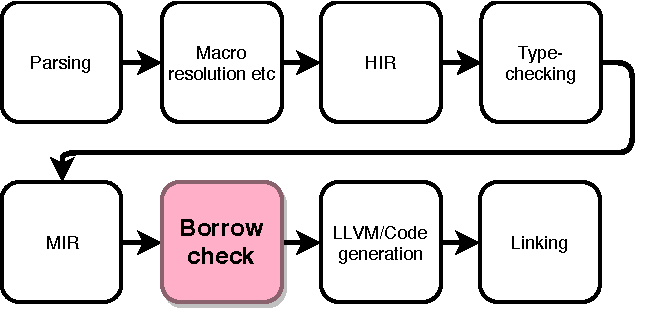
\includegraphics[width=0.9\linewidth]{Graphs/rustc-overview}
  \caption{An overview of the Borrow Check's place in the process of compiling
    Rust code, as described in the Rust Developer's
    Guide~\cite{rustc_developers_guide_nodate}.}
  \label{fig:rustc-overview}
\end{figure}

The logic of the borrow check as described in
Section~\ref{sec:reference-provenance} is calculated at the level of an
intermediate representation of Rust called the Mid-Level Intermediate
Representation (MIR), corresponding to the basic blocks of program control flow.
The input data to the Polonius solver is generated in the Rust compiler by
analysing this intermediate representation. This means that we can safely assume
to be working with simple variable-value assignment expressions, of the type
\InRust{_1 = _2}, as opposed to complex expressions involving multiple variables
on the right-hand side.

\begin{figure}
  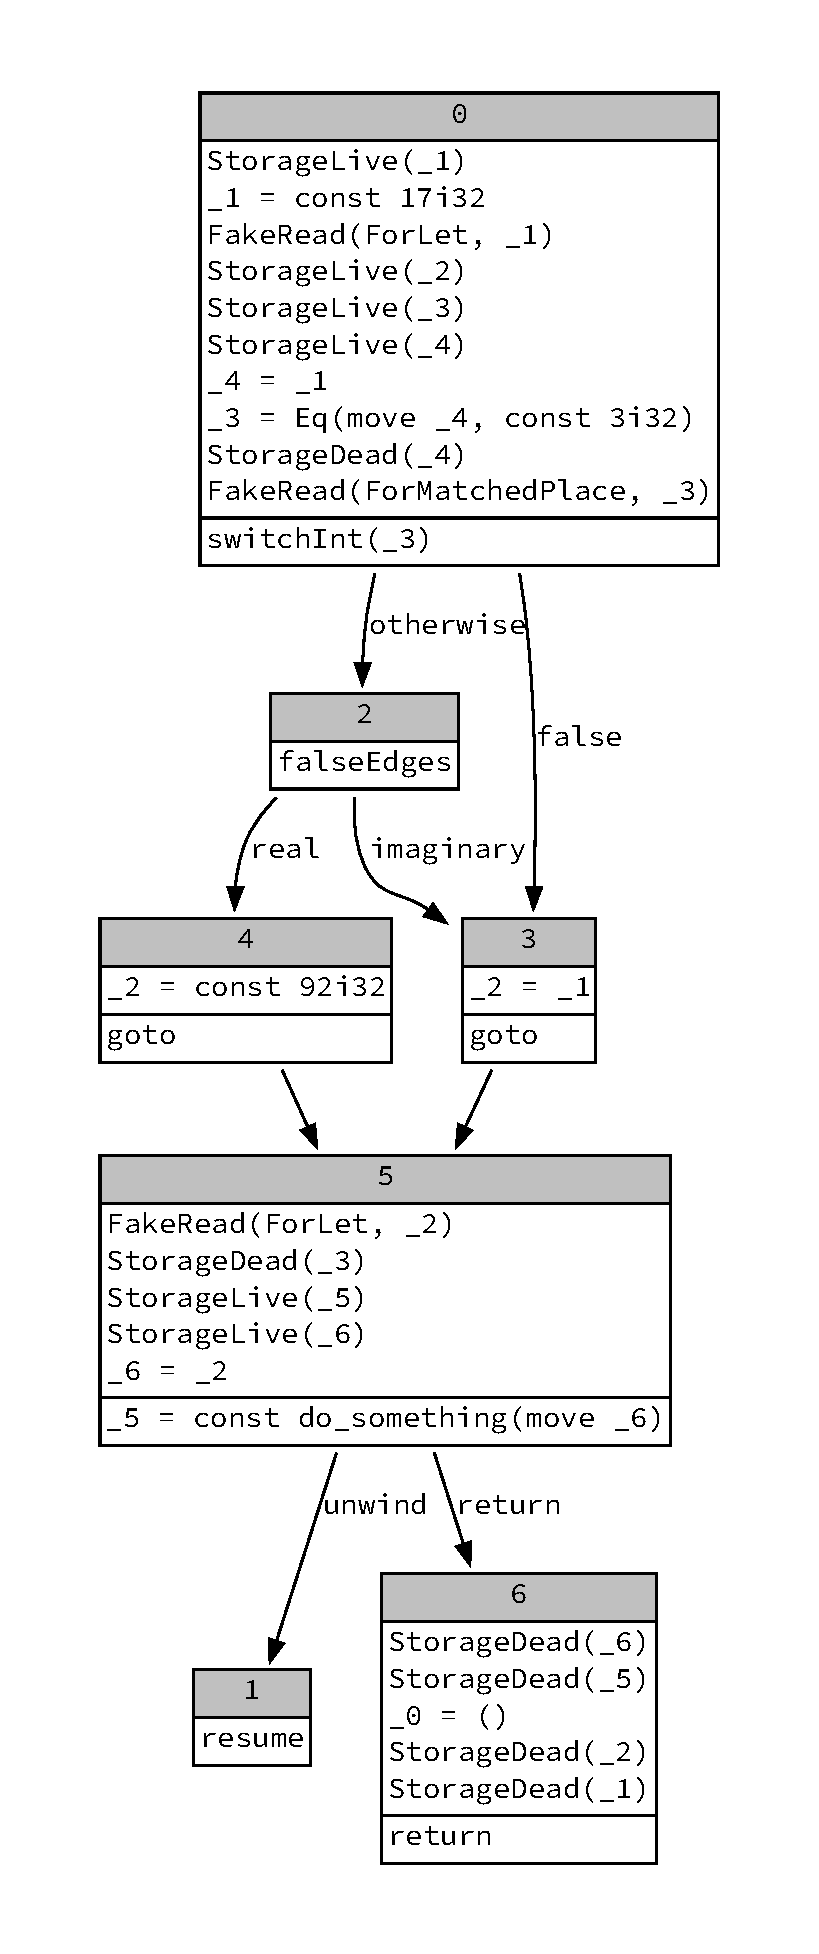
\includegraphics[width=0.65\linewidth]{Graphs/mir-example}
  \caption{A graph rendering of the \InRust{main()} function from the Rust
    program in Listing~\ref{lst:mir-example-input}, illustrating branching
    (block 0), and a function call (5). Note the \texttt{unwind}~arm of block~5's
    terminator (last line), which will be followed if the function call panics.}
  \label{fig:mir-example}
\end{figure}

The MIR consists of basic blocks in the traditional compilers sense, each
containing a set of statements and usually ending with a \emph{terminator}, an
expression providing a branching to other basic
blocks~\cite{mir_rfc,rustc_developers_guide_nodate}. A rendering of the MIR of
the program in Listing~\ref{lst:mir-example-input} can be seen in
Figure~\ref{fig:mir-example}.

\begin{sourcecode}
  \captionof{listing}{A minimal Rust program featuring branching and a function
    call. The MIR~form of this program is shown in
    Figure~\ref{fig:mir-example}.}\label{lst:mir-example-input}
\begin{minted}{rust}
fn main() {
    let x = 17;
    let z = if x == 3 {
        92
    } else {
        x
    };

    do_something(z);
}
\end{minted}
\end{sourcecode}

\section{From Lifetimes to Provenance Variables}
\label{sec:reference-provenance}

As the lifetime of its value is a part of a reference variable's type, it can be
referred to by name like any other type using the syntax \InRust{&'lifetime}. In
the literature, the terms ``region''~\cite{matsakis_alias-based_2018}, ``(named)
lifetime''~\nocite{noauthor_rfc_2019}, and ``reference
provenance''~\cite{weiss_oxide:_2019} (provenance) are all employed. As the
section heading suggests, I will use the last one of them as I believe it best
captures the concept. Named provenances (such as \InRust{'lifetime} above) are
referred to as ``provenance variables''.

From a type system perspective, the provenance is part of the type of any
reference and corresponds to the borrow expressions that might have generated it
in the Polonius formulation of the borrow check. For example, if a reference
\InRust{r} has the type \InRust{&'a Point}, \InRust{r} is only valid as long as
the terms of the loans in \InRust{'a} are upheld. Take for example the code of
Listing~\ref{lst:multi-path-borrow}, where \InRust{p} would have the type
\InRust{&'a i32} where \InRust{a} is the set $\Set{L_0, L_1}$.

\begin{sourcecode}
  \captionof{listing}{An example of a multi-path
    borrow.}\label{lst:multi-path-borrow}
\begin{minted}{rust}
let x = vec![1, 2];

let p: &'a i32 = if random() {
  &x[0] // Loan L0
} else {
  &x[1] // Loan L1
};
\end{minted}
\end{sourcecode}

If a reference is used in an assignment like \InRust{let p: &'b i32 = &'a x},
the reference, \InRust{p}, cannot outlive the assigned value, \InRust{x}. More
formally the type of the right-hand side, \InRust{&'a i32}, must be a subtype of
the left-hand side's type; \InRust{&'a i32 <: &'b i32}. In practice, this
establishes that \InRust{'b} lives at most as long as \InRust{'a}, which means
that the subtyping rules for regions establishes a set membership constraint
between the regions, as seen in Rule~\ref{eq:subtype} of
Section~\ref{sec:type-system}, which gives a brief introduction to the reference
ownership analysis of Polonius from a type system perspective.

Finally, when talking about the \emph{liveness} of a provenance variable $r$ at
some point in the control-flow graph $p$, we will mean that $r$ occurs in the
type of at least one variable which is live at $p$. This has the semantic
implication that any of the loans in $r$ might be dereferenced at control-flow
points reachable from $p$, and thus that the terms of the loans in $r$ must be
respected at that point. For a more formal explanation of this, including an
expansion of how provenance variables are populated, please see the following
section.

\section{Reference Ownership as a Type System}\label{sec:type-system}

In this section, I will summarise the ongoing work of
\citeauthor{weiss_oxide:_2019} on formalising the reference ownership rules of
Rust~\cite{weiss_oxide:_2019} into a type system as it relates to the Polonius
formulation of the borrow checker. At the heart of the type system lies the
flow-sensitive typing judgments seen in Rules~\ref{eq:t-move}
and~\ref{eq:t-borrow}, both of \citeauthor{weiss_oxide:_2019}'s paper
(Figure~1), with slight modifications.

The first rule~\eqref{eq:t-move} shows that for a given environment~$\Gamma$, a
move of a given variable~$\pi$ (occurring if $\pi$ cannot be copied) is only
valid if~$\pi$ is the only name for that value and removes that value from the
environment, effectively deallocating it.

\begin{equation}\label{eq:t-move}
  \ntyperule{\Gamma \vdash_{\text{mut}} \pi : \tau^s \:\: \text{noncopyable } \tau^s}
  {\Sigma ; \Delta ; \Gamma \vdash \expression{\pi} : \tau^s \implies \Gamma - \pi}
  \end{equation}

  The second rule, Rule~\eqref{eq:t-borrow}, tells that we may create an
  $\omega$-reference to any variable where $\omega$-use is safe (either sharedly
  or uniquely), and produce a reference to that variable of the type ``reference
  to a value of $\pi$'s type,~$\tau$, with its provenance variable being the set
  containing only that loan, denoted $^{\omega}\pi$''.

\begin{equation}\label{eq:t-borrow}
  \ntyperule{\Gamma \vdash_{\omega} \pi : \tau}
  {\Sigma ; \Delta ; \Gamma \vdash \expression{\&\omega \pi} : \left \{ ^{\omega}\pi\right \} \omega \tau \implies \Gamma}
\end{equation}

Judgments on the form~$\Gamma \vdash_{\omega} \pi \: : \: \tau$ mean that ``in
the environment~$\Gamma$, it is safe to use the variable~$\pi$ (of type~$\tau$)
$\omega$-ly'' \cite{weiss_oxide:_2019}. In other words, if $\omega$~is
\emph{unique}, it means that there are no live loans of any paths
overlapping~$\pi$, and of $\omega$~is \emph{shared} that there are no
overlapping \emph{unique} loans in the provenance part of $\tau$.

Rules~\eqref{eq:t-move} and~\eqref{eq:t-borrow} constitute ``base cases'' for
the ownership system, showing how variables get removed from the environment,
and how provenance variables in reference types are created. In order to
describe the full analysis, I need to also consider how these relations extend
across program execution through sequencing or branching, of which the latter
introduces the approximate aspect of provenances. Finally, I will also describe
how provenance variables come into relation with each other through type
unification.

Since the borrow check is performed on the MIR, Polonius does not handle
branchings in the normal sense. Therefore, the sequencing and branching rules of
Oxide only translate analogously~\cite{weiss_oxide:_2019}. As in Oxide, the
``type environment'' of the MIR is threaded through the typing of each
expression, such that the sequence of expressions~$\expression{e_1; e_2}$ would
first type-check~$e_1$ and then~$e_2$ in the resulting environment. To capture
this, I will use the name~$\Gamma_p$ to refer to the type-environment mapping
places to their types just before evaluating an arbitrary point~$p$ of the~CFG.

In Oxide, the typing rules for branch expressions provide for a type unification
of the if expression such that its value unifies the provenance variables. The
MIR produced by such a branching would have a loop starting at the head of the
\InRust{if} expression and ending with an assignment to the same variable in
each branch before finally joining in a basic block where the assigned variable
now could have come from either arm. The same unification in Polonius has two
aspects to it: approximation of reference origins, captured by transfer across
CFG edges in the MIR, and type unification, captured on assignment.

Simply put, each assignment allows different types on each side of the
assignment, as long as the types unify, as seen in Rule~\eqref{eq:t-assignment}.
This leads to the same type-unification for references as seen in Oxide
(Rule~\eqref{eq:u-ref}). In practice, this means that each assignment of a
place~$\pi_1$ from another place~$\pi_2$ in the environment~$\Gamma$ updates
$\Gamma$ to have a new mapping such that $\pi_2$'s provenance variable~$\rho_2$
is a superset of $\pi_1$'s.

Finally, in Oxide's \textsc{T-Branch} rule for branching, the type environments
are unified into an approximate type environment that combines provenances in
the variables from each branch. In Polonius, the corresponding logic is simply
that a basic block's starting place-environment~$\Gamma$ is the transitive
closure of the union of the place-environments at the terminators of the
previous blocks.

\begin{equation}\label{eq:t-assignment}
  \ntyperule{\pi_1 : \tau_1 \:\: \pi_2 : \tau_2 \:\: \tau_1 \sim \tau_2 \implies \tau \:\: \Gamma \vdash_{uniq} \pi_1}
  {\Sigma ; \Delta ; \Gamma \vdash \expression{\pi_1 = \pi_2} \: : \: \tau \implies \Gamma - \pi_1, \pi_1 \: : \: \tau}
\end{equation}

\begin{equation}\label{eq:u-ref}
  \ntyperule{\tau_1 \sim \tau_2 \implies \tau \:\:\: \rho_1 \cup \rho_2 = \rho}
  {\&\rho_1 \omega \tau_1 \sim \& \rho_2  \omega \tau_2 \implies \&\rho \omega \tau}
\end{equation}

Under these rules, a Rust function is valid from the perspective of the borrow
check if, for each point in the control flow graph, the borrow rules are
respected. In logic terms, this means that we cannot find a point $p$ in the
control-flow graph such that a loan $\Loan$ is live there while its conditions
are being violated, or more formally $\lnot \exists(\Loan, p) \: : \:
\Live(\Loan, p) \land \Invalidated(\Loan, p))$. These relations are then defined
as follows:
\begin{description}
\item[the $\Live(\Loan, p)$ relation for a loan~$\Loan$] A loan is live at a given
  position $p$ if there exists a live provenance variable $R$ such that $\Loan
  \in R$, or formally: $\exists(\Loan, R, p, \Gamma_p) \: : \: \Live(R, p) \land
  \Loan \in \Gamma_p(R)$, where I by~$\Gamma_p$ mean the environment at $p$,
  and~$\Gamma_p(R)$ mean the loans in~$R$ at point~$p$. \fixme{This is not how
    Weiss uses gamma!}
\item[the $\Live(R, p)$ relation for a provenance variable~$R$] A provenance
  variable is live at~$p$ if and only if a variable whose type it is part of is
  live there. \fixme{type-system describe ``there exists a variable $v$ with
    type $\tau$ such that $R$ is $\tau$'s provenance variable and $\Live(v,
    p)$''}
\item[the $\Live(v, p)$ relation for a variable~$v$] A variable is live at $p$
  if there exists a point~$q$ reachable from~$p$ where $v$ is accessed either
  directly or by a \InRust{drop()} (see Section~\ref{sec:deall-as-spec} for a
  discussion of when a variable is considered to be used in a deallocation),
  without having been overwritten (``killed'') somewhere between $q$ and $p$.
  Notably, a variable is only used by a Drop if it might be partially
  initialised when the drop happens. \fixme{Formalise this.}
\item[the $\MayBeInitialised(v, q)$ relation for a variable~$v$] A variable may
  be (partially) initialised if there is a path through the CFG from a point
  $p$, where some part $\pi$ of $v$ is initialised, to $q$ without $\pi$ getting
  deallocated along that path. \fixme{Formalise this.}
\item[$\Loan \in R$ for loan $\Loan$] A loan is a member of $R$ if and only if is
  was originally part of the loan that created $R$, or if $\exists R' \: :
  \:\Loan \in R' \land R' \subseteq R$. \fixme{Describe relationship to gamma!}
  \fixme{How to point-qualify these relationships?}
  \item[$R' \subseteq R$ for provenance variables $R, R'$] \fixme{write this}
\end{description}

\section{Deallocation As a Special Case of Variable Use}
\label{sec:deall-as-spec}
When Rust's variables go out of scope, they are implicitly deallocated, or
dropped in Rust parlance. Explicit deallocation is also possible by calling the
function \InRust{drop()}, which takes ownership of a variable (that is,
deinitialises it) and performs deallocation, or, for complex objects, calls the
\InRust{drop()} method. For some types such as integers, deallocation is not
necessary and the compiler generates no actual \InRust{drop()}:s in the MIR.

Rust provides a default deallocator for data structures, but it can be
overridden. This has repercussions on liveness calculations, because while the
default deallocator for an object never needs to access its fields except to
deallocate them, a custom deallocator might access any of them in arbitrary
ways. This means that any conditions of a loan that resulted in a reference $r$
stored in a \InRust{struct} $s$ instance $a$ must only be respected as far as
\InRust{a.drop()} is concerned if $s$ implements a custom deallocator. Otherwise
the loan of $r$ may be safely violated, as the default deallocator never
dereferences $r$ and thus doesn't require $r$ to be valid. An illustration of
this can be seen in Listing~\ref{lst:drop-liveness}.

\begin{sourcecode}
  \captionof{listing}{The custom deallocator for \InRust{OwnDrop} enforces the
    loan of \InRust{data}, but the loan in \InRust{OwnDrop} is effectively dead
    and thus can be violated.}\label{lst:drop-liveness}
\begin{minted}{rust}
struct OwnDrop<'a> {
    data: &'a u32,
}

struct DefaultDrop<'a> {
    data: &'a u32,
}

impl<'a> Drop for OwnDrop<'a> {
    fn drop(&mut self) {
        // might access self.data
    }
}

fn main() {
    let mut x = 13;
    let a = OwnDrop { data: &x };

    let mut y = 12;
    let b = DefaultDrop { data: &y };
    
    // let mutrefa = &mut x;
    // ERROR: the loan of x must be respected...
    
    // ...but the loan of y need not be!
    let mutref = &mut y;
    *mutref = 17;
    
    // all variables are implicitly dropped here
}
\end{minted}
\end{sourcecode}

\section{Datalog and Datafrog}
\label{sec:datalog}

Datalog is a derivative of the logic programming language Prolog, with the
desirable properties that any program terminates in polynomial time, and in some
variants also with the power to express all polynomial-time
computation~\cite{afrati_datalog_1995}. It describes fixpoint calculations over
logical relations as predicates, described as fixed input \emph{facts}, computed
\emph{relations}, or \emph{rules} describing how to populate the relations based
on facts or other relations. For example, defining a fact describing that an
individual is another individual's parent might look like
\InDatalog{parent(mary, john).}, while computing the \InDatalog{ancestor}
relation could then use the two rules, reflecting the fact that ancestry is
respectively either direct parenthood or transitive parenthood (example from the
Wikipedia article on Datalog~\cite{wiki:datalog}):
\begin{minted}{rust}
ancestor(X, Y) :- parent(X, Y).
ancestor(X, Y) :- parent(X, Z), ancestor(Z, Y).
\end{minted}

Datafrog~\cite{datafrog} is a minimalist Datalog implementation embedded in
Rust, providing an implementation of a worst-case optimal join algorithm as
described in~\cite{ngo_worst-case_2012}. The fact that Datafrog is embedded in
Rust means that standard Rust language abstractions are used to describe the
computation. Static facts are described as \InRust{Relation}s, while
\InRust{Variable}s are used to capture the results of computations, both of
which are essentially sets of tuples. Rules are described using a join with
either a \InRust{Variable} or a \InRust{Relation}, with an optimised join
method for joins with the variable itself. Only single-step joins on the first
tuple element are possible, which means that more complex rules must be written
with intermediary variables, and manual indices created whenever a relation must
be joined on a variable which is not the first in the tuple.

\begin{sourcecode}
  \captionof{listing}{The implementation of \InDatalog{var_live(V, P)} in
    Datafrog.}\label{lst:datafrog:var-live}
\begin{minted}{rust}
var_live_var.from_leapjoin(
    &var_live_var,
    (
        var_defined_rel.extend_anti(|&(v, _q)| v),
        cfg_edge_reverse_rel.extend_with(|&(_v, q)| q),
    ),
    |&(v, _q), &p| (v, p),
);
\end{minted}
\end{sourcecode}


As an example, the Datafrog code for \InDatalog{var_live(V, P)} of
Listing~\ref{lst:var-live} becomes the code in
Listing~\ref{lst:datafrog:var-live}, and the corresponding join used for the
first half of \InDatalog{region_live_at(R, P)} of
Listing~\ref{lst:region-live-at} can be seen in
Listing~\ref{lst:datafrog:region-live-at}.

\begin{sourcecode}
  \captionof{listing}{The first half of the implementation of
    \InDatalog{region_live_at(R, P)} in
    Datafrog.}\label{lst:datafrog:region-live-at}
\begin{minted}{rust}
region_live_at_var.from_join(
    &var_drop_live_var, 
    &var_drops_region_rel, 
    |_v, &p, &r| {
        ((r, p), ())
    });
\end{minted}
\end{sourcecode}

Joins in Datafrog are done using one of two methods on the variable that is to
be populated (e.g. in Listing~\ref{lst:datafrog:region-live-at}
\InRust{region_live_at_var}), a variable with tuples of the format \InRust{(Key,
  Val1)}. The first method, \InRust{from_join}, performs simple joins from
variables or relations into the (possibly different) target variable. Its
arguments, in order, are a \InRust{Variable} of type \InRust{(Key, Val2)}, and
either a second \InRust{Variable} or a \InRust{Relation} of type \InRust{(Key,
  Val3)}. The third and final argument is a combination function that takes each
result of joining the two non-target arguments, a tuple of type \InRust{(Key,
  Val2, Val3)}, and returns a tuple of format \InRust{Key, Val1} to be inserted
into the target variable.

For more complex joins where a single variable participates in the join and all
other arguments are static \InRust{Relation}s (such as is the case with the
variable~\InRust{var_live_var} of Listing~\ref{lst:datafrog:var-live}), there is
\InRust{from_leapjoin}. In this case, the input is the sole dynamic source
variable, a tuple of ``leapers'', and a combining function like the one in
\InRust{from_join}, but with the signature like the one above, mapping a matched
tuple from the join to the target of the join.

A leaper is created from a \InRust{Relation} of type \InRust{(Key, Value)} by
either applying the method \InRust{extend_with} or \InRust{extend_anti} for a
join or an anti-join respectively. Both of these functions then take a function
mapping tuples from the \InRust{Variable} to \InRust{Key}s in the
\InRust{Relation} being (anti-)joined. In the case of \InRust{extend_anti}, any
tuples matching \InRust{Key} are discarded.


In this thesis, I will use the notation of Souffl{\'e}~\cite{scholz_fast_2016}
for all examples for clarity and brevity, even though the actual code was
written in Datafrog.

\chapter{A Declarative Model for the Rust Borrow Checker}
\label{cha:investigation}
% \epigraph{\fixme{short quote}}

\section{The Borrow Checker in Datalog}\label{sec:borr-check-datal}

\subsection{Starting Facts}
\label{sec:input-facts}

The following short-hand names are used:
\begin{description}
\item[$R$] is a provenance.
\item[$L$] is a loan, that is an \InRust{&v} expression creating a reference
  to \InRust{v}.
\item[$P, Q$] are points in the control-flow graph of the function under analysis.
\item[$V$] is a variable.
\item[$M$] is a Move Path, that is a part of a variable that can be accessed
  and, more importantly, deinitialised. This can be the name of a variable (e.g.
  \InRust{a}), or an access of a field of a data structure or one of a tuple's
  projections (e.g. \InRust{a.b}, or \InRust{a.1}).
\end{description}


\begin{description}
\item[\InDatalog{borrow_region(R, L, P)}] the provenance~$R$ may refer
  to data from loan $L$ starting at the point $P$ (this is usually the point
  \emph{after} the right-hand-side of a borrow expression).
  
\item[\InDatalog{universal_region(R)}] for each named/parametrised provenance
  variable~$R$ supplied to the function. $R$ is considered universally
  quantified, and therefore live in every point of the function.
  
\item[\InDatalog{cfg_edge(P, Q)}] whenever there is a transition~$P \rightarrow
  Q$ in the control flow graph.
    
\item[\InDatalog{killed(L, P)}] when some prefix of the path (\fixme{explain
    prefixes and paths}) borrowed in $L$ is assigned at point~$P$.
    
\item[\InDatalog{outlives(R1, R2, P)}] when $R_1 \subseteq R_2$ must hold at
  point~$P$, a consequence of subtyping relationships as described in
  Rule~\eqref{eq:subtype}.
    
\item[\InDatalog{invalidates(P, L)}] when the loan~$L$ is invalidated by some
  operation at point~$P$.
    
\item[\InDatalog{var_used(V, P)}] when the variable~$V$ is used for anything but
  a drop at point~$P$.
    
\item[\InDatalog{var_defined(V, P)}] when the variable~$V$ is assigned to
  (killed) at point~$P$.
  
\item[\InDatalog{var_drop_used(V, P)}] when the variable~$V$ is used in a drop at point~$P$.

\item[\InDatalog{var_uses_region(V, R)}] when the type of~$V$ includes the
  provenance~$R$.

\item[\InDatalog{var_drops_region(V, R)}] when the type of~$V$ includes the
  provenance~$R$, and~$V$ also implements a custom drop method which might need
  all of~$V$'s data, as discussed in Section~\ref{sec:deall-as-spec}.
\end{description}


\fixme{Update this list for initialisation tracking!}

\subsubsection{Emitting Facts from the Rust Compiler}\label{sec:sec-rustc-fact-generation}

\fixme{A nice illustration of where we hook into the code and what happens there}

\fixme{A description of how and where facts are generated.}

\subsection{Variable Initialisation}
\label{sec:var-initalisation}

\subsubsection{Reporting Initialisation Errors}
\label{sec:initialisation:errors}

\subsection{Reference Liveness}
\label{sec:var-livenes}

The basic liveness of a variable (Listing~\ref{lst:var-live}) is defined as
follows: if a variable~$v$ is live in some point~$q$ and~$q$ is reachable from
$p$ in the control-flow graph, then~$v$ is live in~$p$ too unless it was
overwritten; in essence liveness is propagated backwards through the CFG.

\begin{sourcecode}
  \captionof{listing}{The Datalog rules for variable
    use-liveness.}\label{lst:var-live}
\begin{minted}{prolog}
var_live(V, P) :-
    var_live(V, Q),
    cfg_edge(P, Q),
    !var_defined(V, P).
\end{minted}
\end{sourcecode}

\fixme{describe drop-liveness}

There is also a very similar relation for drop-liveness with an identical shape
and different input relations corresponding to drop-uses. An example of the
output from this calculation can be seen in Figure~\ref{fig:liveness-graph}.

Both of these are then used to calculate the reference liveness relation
(Listing~\ref{lst:region-live-at}), which serves as input for the rest of the
borrow checker. A given provenance~$r$ is live at some point~$p$ if it is in the
type of a variable~$v$ which is either drop-live or use-live at~$p$, with some
notable caveats for drop-liveness (discussed in Section~\ref{sec:deall-as-spec})
embedded in the \InDatalog{var_drops_region} relation.

\begin{sourcecode}
  \captionof{listing}{The Datalog rules for provenance
    liveness.}\label{lst:region-live-at}
\begin{minted}{prolog}
region_live_at(R, P) :-
    var_drop_live(V, P),
    var_drops_region(V, R).
        
region_live_at(R, P) :-
        var_live(V, P),
        var_uses_region(V, R).
\end{minted}
\end{sourcecode}

\begin{figure}
  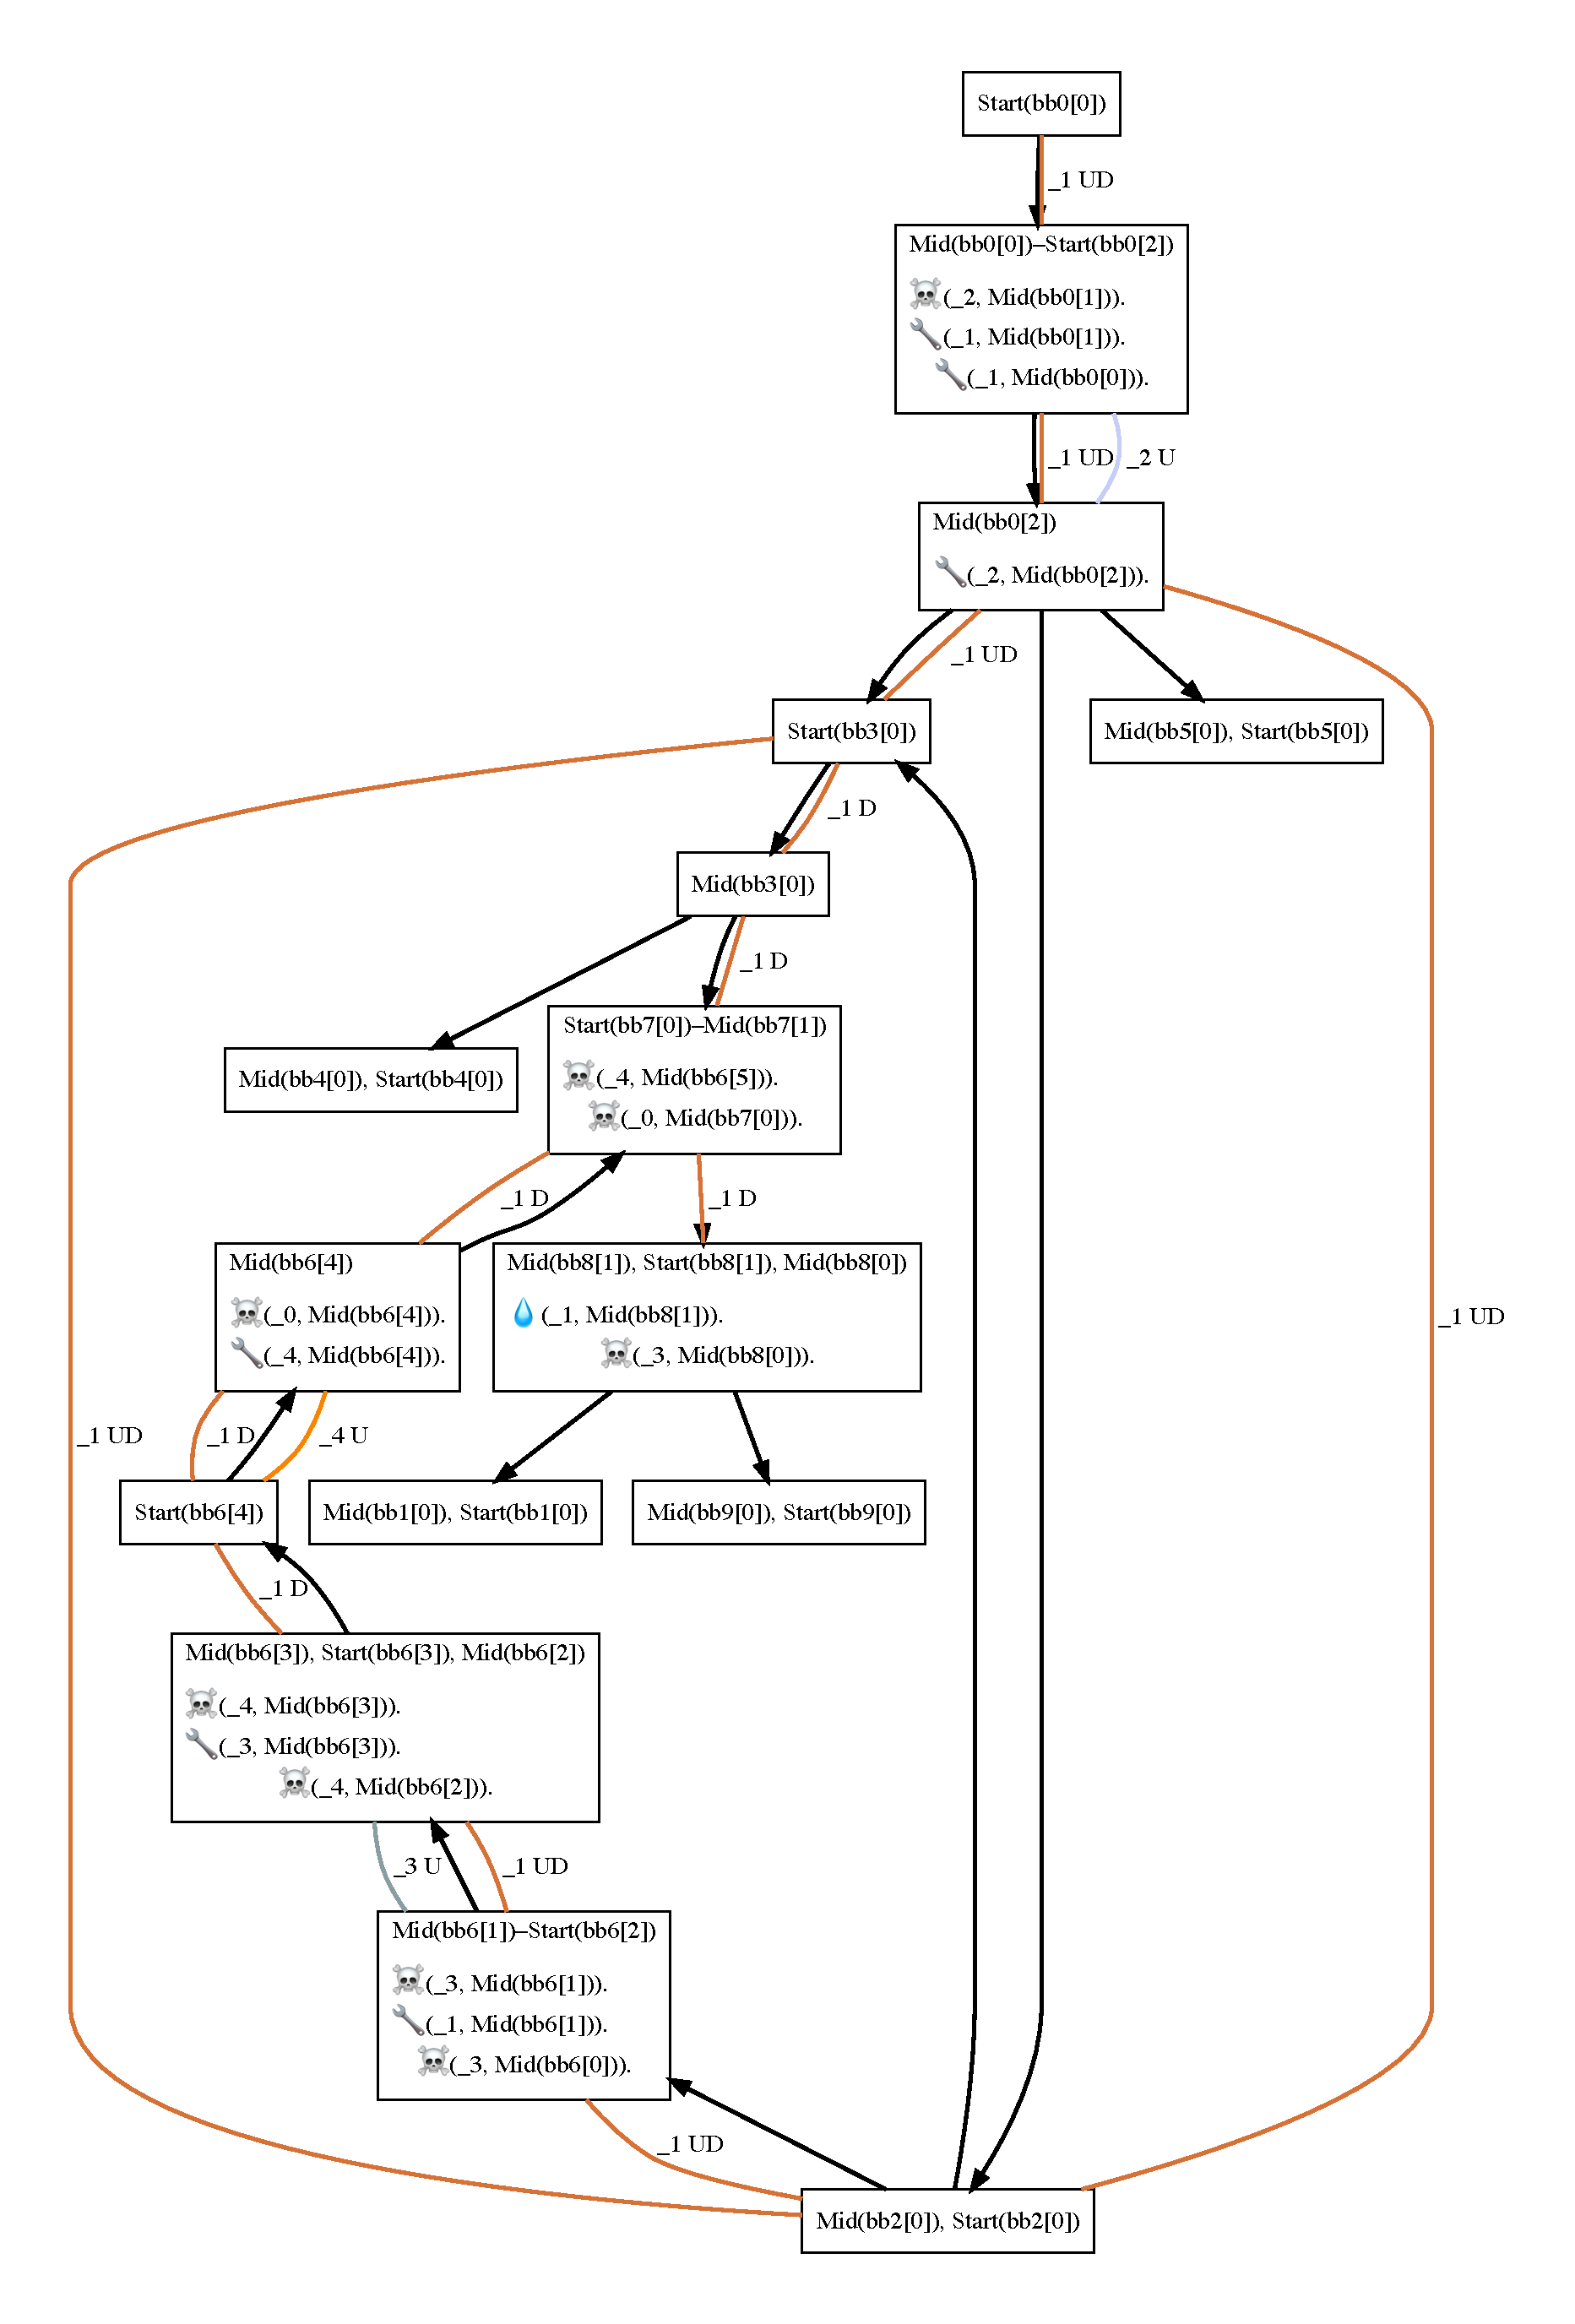
\includegraphics[width=0.9\linewidth]{Graphs/liveness.pdf}
  \caption{A graph representation of the the variable liveness calculation
    results, with relevant Polonius facts as they occur (a droplet symbolising
    \InDatalog{var_drop_used}, a wrench \InDatalog{var_used}, and a skull and
    crossbones symbolising \InDatalog{var_defined}). Variables are named by
    prefixing underscores, and edges annotated with the propagated live variable
    and its liveness type(s) (\textbf{D}rop or \textbf{U}se).}
  \label{fig:liveness-graph}
\end{figure}

\subsection{Loan Constraint Propagation\notmine{}}\label{sec:loan-constr-prop}

The first relation used in Polonius is the \InDatalog{subset(R1, R2, P)}
relation, which states that~$R_1 \subseteq R_2$ for two provenance
variables~$R_1, R_2$ at point~$p$ in the CFG. Initially, these have to hold at
the points where the constraints are generated by the Rust compiler, as seen by
the input parameter~\InDatalog{outlives}. The brief one-liner in
Listing~\ref{lst:subset-outlives} captures this fact, providing a ``base case''
for the computation. Additionally, subset relations are transitive, which is
captured in Listing~\ref{lst:subset-transitive}.

\begin{sourcecode}
  \captionof{listing}{Subset relations hold at the point where they are
    introduced.}\label{lst:subset-outlives}
\begin{minted}{prolog}
subset(R1, R2, P) :- outlives(R1, R2, P).
\end{minted}
\end{sourcecode}

\begin{sourcecode}
  \captionof{listing}{Subset relations are transitive.}\label{lst:subset-transitive}
\begin{minted}{prolog}
subset(R1, R3, P) :-
    subset(R1, R2, P),
    subset(R2, R3, P).
\end{minted}
\end{sourcecode}

Finally, Polonius needs logic to carry these subset relations across program
flow. Recalling the rules of \fixme{which ones? refer back to the theory here},
a subset relation should be propagated across an edge of the control-flow graph
if and only if its provenance variables are live, otherwise we are in a ``if a
tree falls in the woods'' situation where the conditions of the loans can be
safely violated as there is no live reference to be affected. Therefore, the
rule for propagating the subset constraint across a CFG~edge $P \rightarrow Q$
becomes the formulation seen in Listing~\ref{lst:subset-propagation}, which
notably uses the output of the liveness calculations described in
Section~\ref{sec:var-livenes}.

\begin{sourcecode}
  \captionof{listing}{Subset relations propagate across CFG~edges iff their
    provenance variables are live.}\label{lst:subset-propagation}
\begin{minted}{prolog}
subset(R1, R2, Q) :-
    subset(R1, R2, P),
    cfg_edge(P, Q),
    region_live_at(R1, Q),
    region_live_at(R2, Q).
\end{minted}
\end{sourcecode}

These rules describe how provenance variables relate to each other. The other
part of the logic describes which loans belong to which provenance variable. The
trivial base case is shown in Listing~\ref{lst:requires-borrow}, which just says
that each provenance variable~$R$ contains the loan~$L$ that created it at point
the point~$P$ where the borrow occurred.

\begin{sourcecode}
  \captionof{listing}{A provenance variable trivially contains
    (\InDatalog{require}s) the loan which introduced
    it.}\label{lst:requires-borrow}
\begin{minted}{prolog}
requires(R, L, P) :- borrow_region(R, L, P).
\end{minted}
\end{sourcecode}

Additionally, the \InDatalog{requires}~relation needs to be propagated together
with subset constraints; after all $R_1 \subseteq R_2$ implies that $R_2$ must
contain (\InDatalog{require}) all of $R_1$'s~loans. This is captured by the rule
in Listing~\ref{lst:requires-subset}.

\begin{sourcecode}
  \captionof{listing}{A subset relation between two provenance variables $R_1$,
    $R_2$ propagates the loans of $R1$ to $R2$.}\label{lst:requires-subset}
\begin{minted}{prolog}
requires(R2, L, P) :- 
  requires(R1, L, P), 
  subset(R1, R2, P).
\end{minted}
\end{sourcecode}

Finally, Polonius performs the flow-sensitive propagation of these membership
constraints across edges in the CFG. This is done using the rule in
Listing~\ref{lst:requires-edge}, where the requirements propagate across
CFG~edges for every loan~$L$ as long as the reference corresponding to~$L$ is
not overwritten (\InDatalog{killed}), and only for provenance variables that are
still live. Recall \fixme{(from where?)} that loans are uniquely tied to one
point in the CFG, and therefore to a single place. This is why a single loan is
killed by a single assignment.

\begin{sourcecode}
  \captionof{listing}{Propagate loans across CFG edges for live provenance
    variables and loans whose references are not
    overwritten.}\label{lst:requires-edge}
\begin{minted}{prolog}
requires(R, L, Q) :-
  requires(R, L, P),
  !killed(L, P),
  cfg_edge(P, Q),
  region_live_at(R, Q).
\end{minted}
\end{sourcecode}


\subsubsection{Detecting Loan Violations}

The compiler produces a set of points in the CFG where a loan could possibly be
violated (e.g. by producing a reference to a value that already has a unique
reference) in \InDatalog{invalidates}. All that remains for Polonius is to
figure out which loans are live where (Listing~\ref{lst:loan-live}), and see if
any of those points intersect with an invalidation of that loan
(Listing~\ref{lst:error-invalidates}).

\begin{sourcecode}
  \captionof{listing}{Loans are live when their provenance variables
    are.}\label{lst:loan-live}
\begin{minted}{prolog}
loan_live_at(L, P) :-
  region_live_at(R, P),
  requires(R, L, P).
\end{minted}
\end{sourcecode}

\begin{sourcecode}
  \captionof{listing}{It is an error to invalidate a live
    loan.}\label{lst:error-invalidates}
\begin{minted}{prolog}
error(P) :-
  invalidates(P, L),
  loan_live_at(L, P).
\end{minted}
\end{sourcecode}

\subsection{Illegal Subset Relations}\label{sec:illeg-subs-relat}

\fixme{this isn't implemented yet!!!}

\section{Generating Facts for Polonius in the Rust Compiler}

\fixme{say something about how and when the facts are generated in the Rust
  compiler.}

\section{A Field Study of Polonius Inputs}\label{sec:field-study-borrow}

I selected roughly 20 000~publicly available Rust packages (``crates'') from the
most popular projects, as defined by number of downloads from Crates.io and
number of stars on GitHub, for analysis.~\footnote{Source code for the analysis
  as well as listings of the repositories are available at
  \url{https://github.com/albins/msc-polonius-fact-study}.} Of the initially
selected repositories only about 1 000 were from other sources than GitHub. Only
crates that compiled under recent versions of Rust nightly builds with
non-linear lifetimes enabled were kept. The source code of the packages was then
translated to Polonius input files for a total of 400GBs~of tab-separated tuples
for 3~077~887~functions, which I used to measure Polonius solve-time performance
as well as for finding common patterns in the input data. Only complete data
sets were considered; a repository with more than one target where at least one
target did not compile was discarded, as was any repository where the analysis
took more than 30~minutes, required more memory than what was available, or
where fact generation took longer than $30$~minutes. After this selection
process, 10~613~repositories remained for the final study, each of which
contained at least one, but possibly multiple crates. It is worth mentioning
that the analysis assumed that all functions in all crates and all targets of a
repository were unique, as the outputs were stored per-repository. The median
number of functions in the dataset was 47, including functions generated by
desugaring as well as user-written functions.

It is worth pointing out that Polonius' analysis as part of the Rust compiler
will be performed on non-compiling Rust code as well, and that the requirement
that all crates must compile is an entirely artificial one and might exclude
interesting input cases. However, it is non-trivial to separate build failures
due to syntax errors or missing dependencies from build failures at later stages
of the build process that would involve Polonius. Therefore all non-compiling
crates were excluded from the study.

Additionally, I also excluded all functions that had no loans at all from the
analysis, a surprisingly large portion; almost 47\%. This is most likely due to
code generation producing short ``functions'' that does not actually involve any
borrowing at all.

The main metric of ``performance'' in this study is the time it would take
Polonius to solve a given set of inputs. In this case, this also includes the
time it takes to parse the files of tab-separated input tuples, which is assumed
to be negligible compared to the runtime of the analysis itself, which includes
both a liveness analysis and the borrow check itself. In practical scenarios the
peak memory usage of the analysis would also be an interesting metric.

When studying inputs to Polonius, I am mainly interested in two properties; how
large and how complex the function under analysis is. Neither of these can be
measured directly, but useful proxy variables would be sizes of input tuples,
the number of variables, loans, and regions, as well as common and cheaply
computed graph complexity metrics such as the node count, density, transitivity,
and number of connected components of the control-flow graph.

Three variants of Polonius were included in the study; a \textsc{Naive}
implementation, which is the one described in
Section~\ref{sec:borr-check-datal}, an optimised variant (\textsc{DatafrogOpt}),
and a variant that first executes a simpler analysis assuming lexical lifetimes
and falls back to the full Polonius analysis only when that one produces an
error (\textsc{Hybrid}). The intention is to have such a hybrid algorithm re-use
the information gained by the simpler analysis to accelerate the more advanced
analysis, but such functionality was not yet implemented at the time of the
experiments.

\begin{figure}
  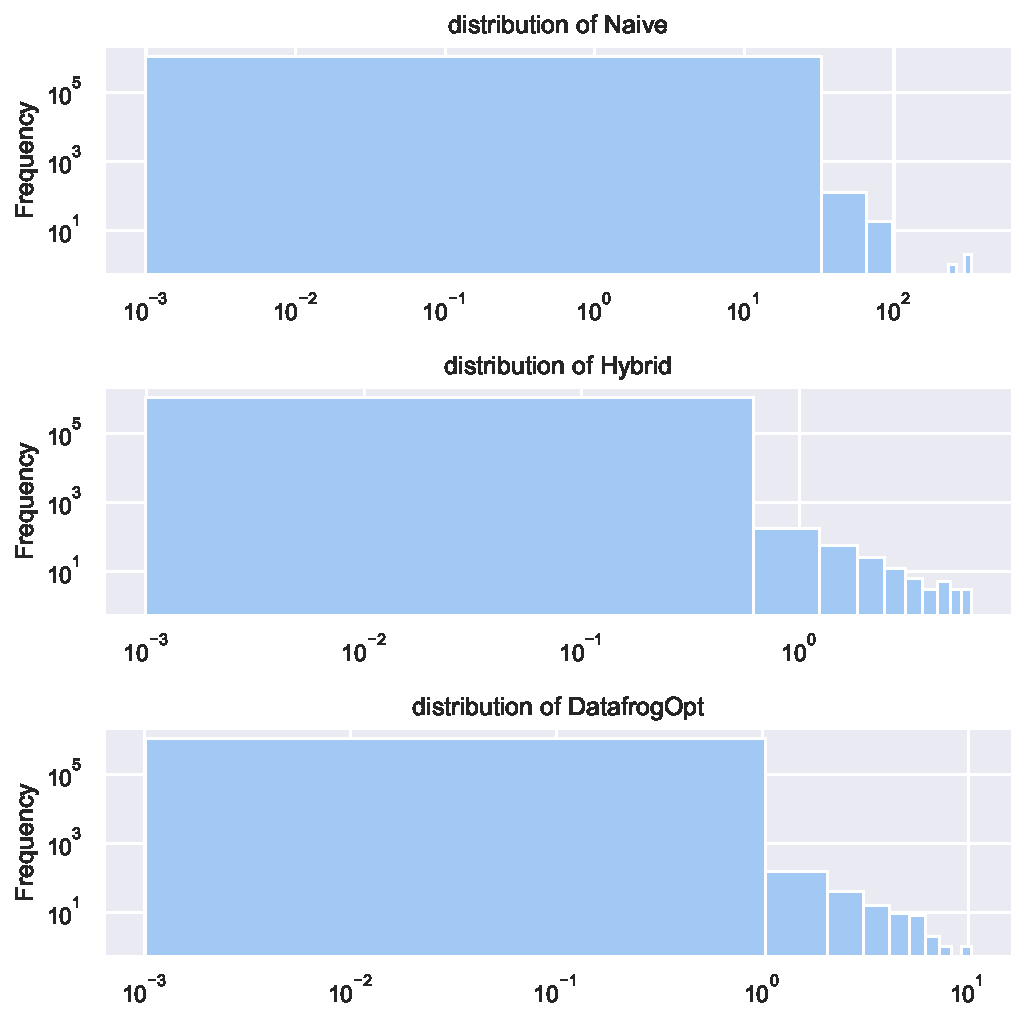
\includegraphics[width=0.9\linewidth]{Graphs/solvetimes_dist.pdf}
  \caption{Distributions of solve-times per function for three implementations
    of Polonius. As can be seen here, the vast majority execute very quickly.}
  \label{fig:solvetimes}
\end{figure}

\subsection{Performance}\label{sec:inputs:performance}

In general, all three algorithms finished quickly for almost all functions, with
both of the optimised algorithms already showing improvements in
solve-times, as seen in Figure~\ref{fig:solvetimes}. Apparently, \textsc{Naive}
has an even tighter spread of solve-times than the others. Additionally,
geometric means of the observed solve-times show improvements from hybridisation
(Figures~\ref{fig:solvetimes-gmean-fn} and~\ref{fig:solvetimes-gmean-repo}),
though it should be noted that the algorithm's worst-case of an input that fails
both the simple and the full analysis was left out of the sample as that would
have failed compilation, possibly inflating the results.

\begin{figure}
  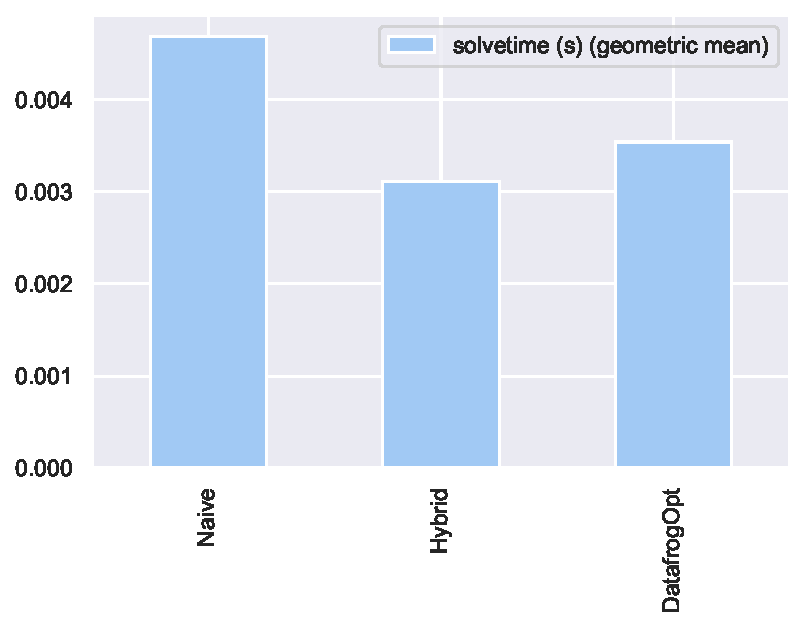
\includegraphics[width=0.5\linewidth]{Graphs/solvetimes_fn_gmean.pdf}
  \caption{Geometric means of the solve-times per function and implementation.}
  \label{fig:solvetimes-gmean-fn}
\end{figure}


\begin{figure}
  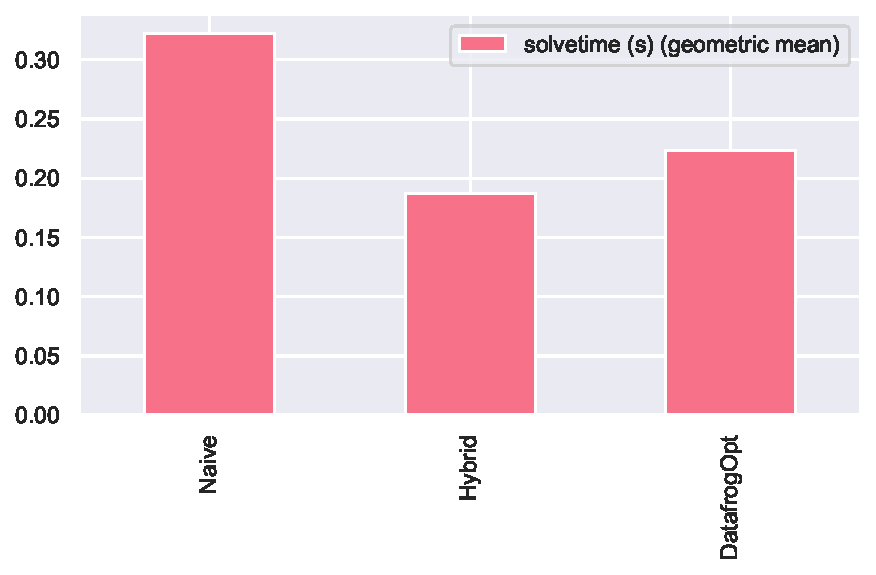
\includegraphics[width=0.5\linewidth]{Graphs/solvetimes_repo_gmean.pdf}
  \caption{Geometric means of the solve-times per repositoriy and
    implementation.}
  \label{fig:solvetimes-gmean-repo}
\end{figure}


\subsection{What is a Typical Input?}\label{sec:inputs:inputs}

\begin{figure}
  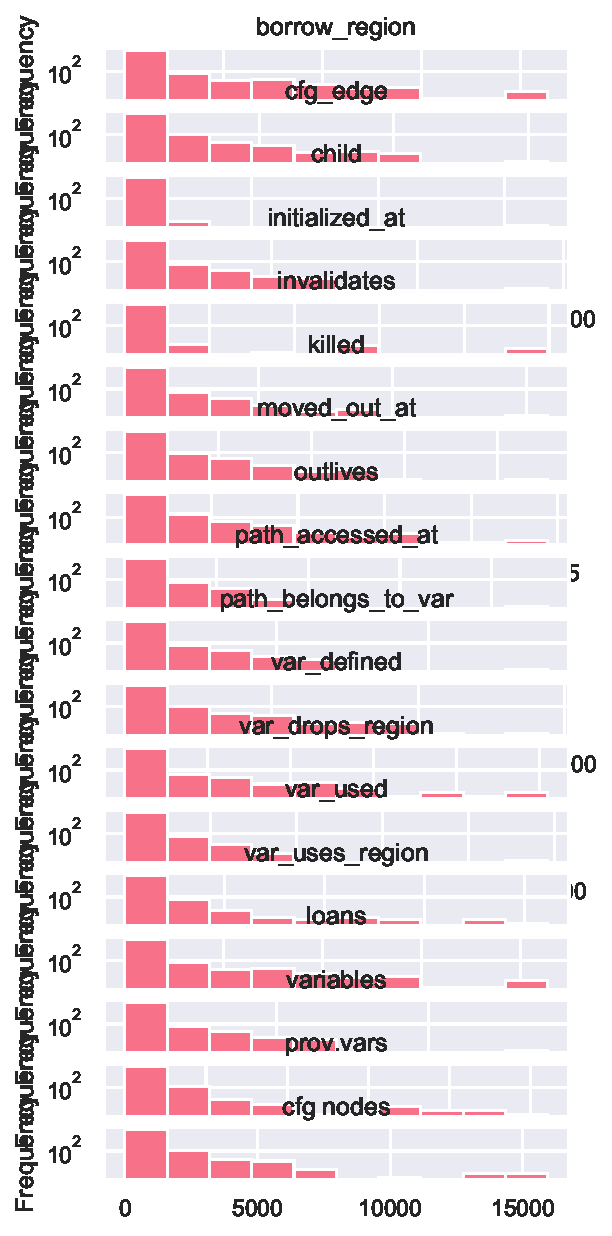
\includegraphics[width=0.5\linewidth]{Graphs/input_sizes_dist.pdf}
  \caption{Distribution of the various input sizes.}
  \label{fig:input-sizes}
\end{figure}

A typical Polonius input consists of a small number of tuples for most
relations, as seen in Figure~\ref{fig:input-sizes}. In particular, most
control-flow graphs are small in terms of number of nodes, and most functions
only contain a small number of variables, with an even smaller number of loans.
Drops are particularly rare, with 71\% of all studied functions having no
(potential) drop-uses at all (0 median, 3.6 mean), and only very few loans
(2~median, 5.4~mean).

This points towards a need to have a low starting overhead for Polonius, as
much of its analysis would have to be performed on very small inputs, where the
solve-time would be dominated by any high constant setup time.

However, repositories can be assumed to be typically compiled all at once.
Therefore, it is also interesting to say something about the maximum input size
per repository, under the assumption that few large functions would dominate the
solve-time for that repository. After collecting the maximum values per repository,
the median number of loans was 24, and the median number of potential drop-uses
was 20 (regular uses was, for comparison, 174).

I attempted to perform a principal-component analysis (PCA) of the input data in
order to visually identify possible clusterings of types of inputs, but the
results were unusable as the inputs had no visually discernible patterns in
neither 2 nor 3 dimensions, suggesting that most inputs are ``typical''.

\subsection{How Inputs Affect Solve-Time}\label{sec:inputs:correlation}

A heatmap of the (Pearson) correlation between input size and solve-time for the
various variants can be seen in Figure~\ref{fig:corr-heatmap}, while a scatter
plot of the results with a linear regression for some interesting pairs of
inputs can be seen in Figure~\ref{fig:input-scatter}.

\begin{figure}
  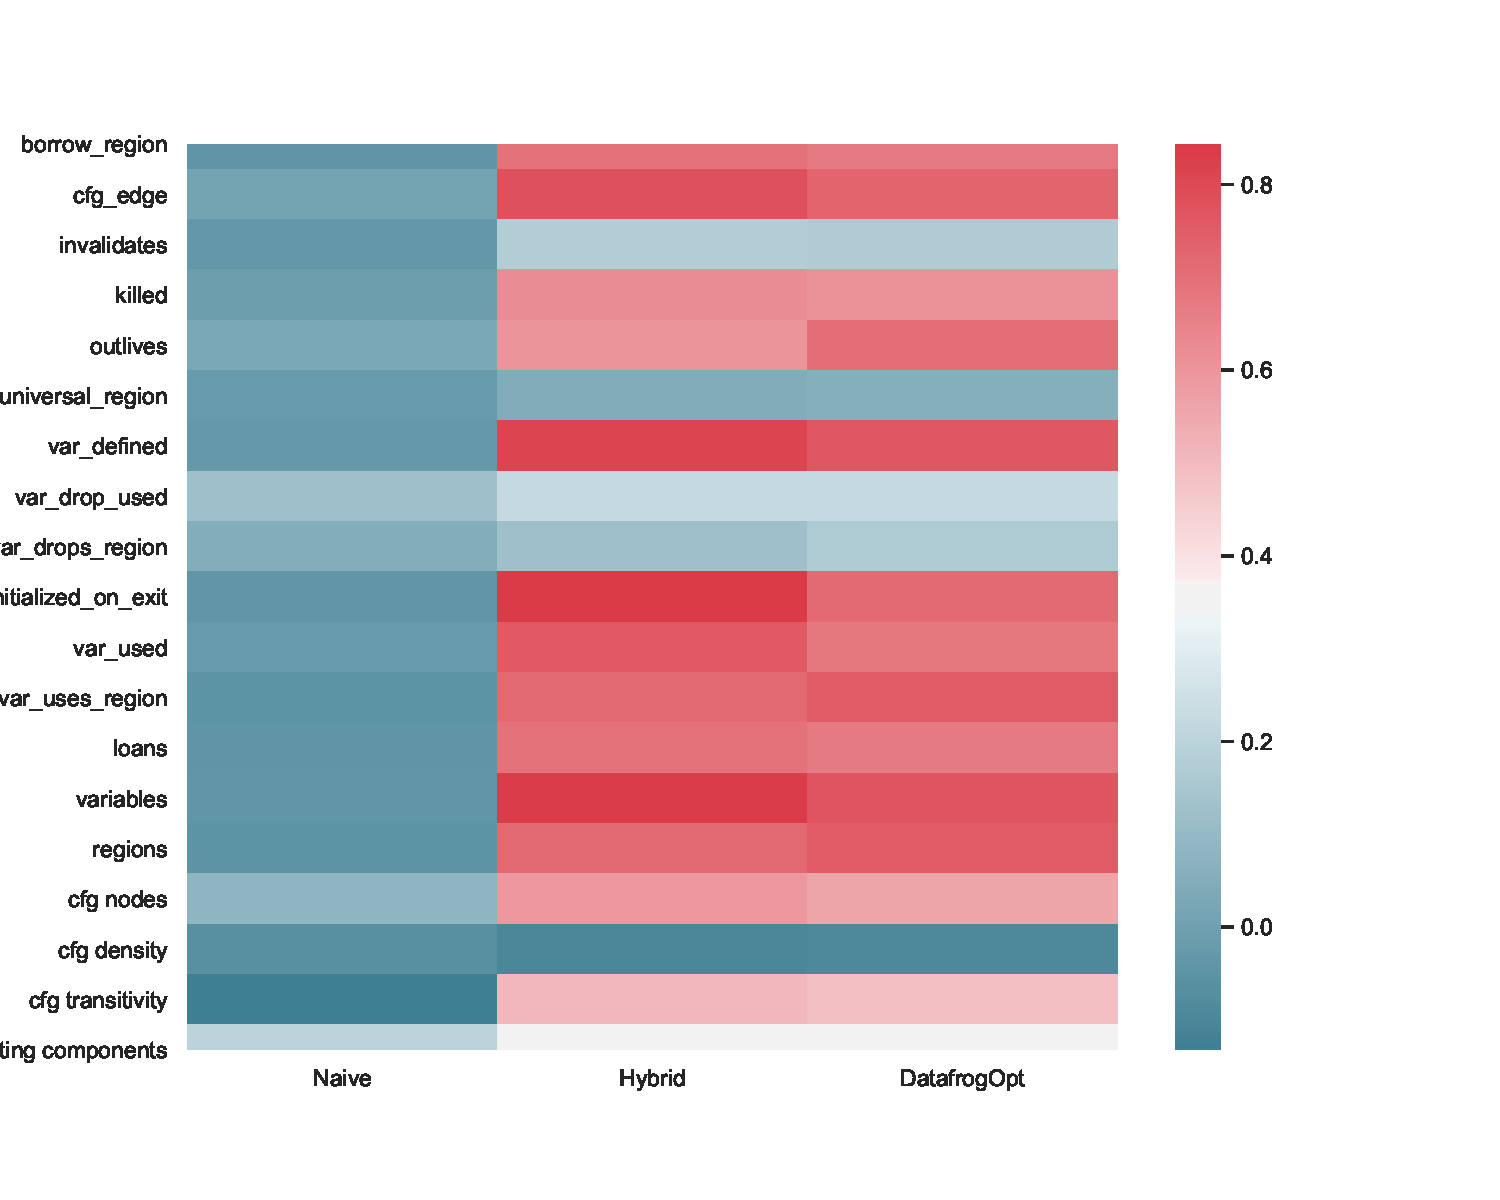
\includegraphics[width=0.9\linewidth]{Graphs/corr_heatmap.pdf}
  \caption{Heatmap of Pearson~correlations between various input size metrics
    and solve-times for all three Polonius implementations, suggesting that in
    particular the number of variables and size of the CFG affect solve-time.}
  \label{fig:corr-heatmap}
\end{figure}

Both results suggest only a very weak linear relation between input sizes and
and the solve-time with the naive algorithm, while a clearer relation can be
found between the two optimisations and input sizes respectively. In particular,
the number of loans and number of nodes in the control-flow graph seems to
affect runtime performance, which is hardly surprising: the number of CFG~nodes
(along with the number of variables) would affect how many times constraint
propagation would happen, and the number of loans and variables would affect the
size of the propagations for the borrow check and liveness analyses
respectively.

\begin{figure}
  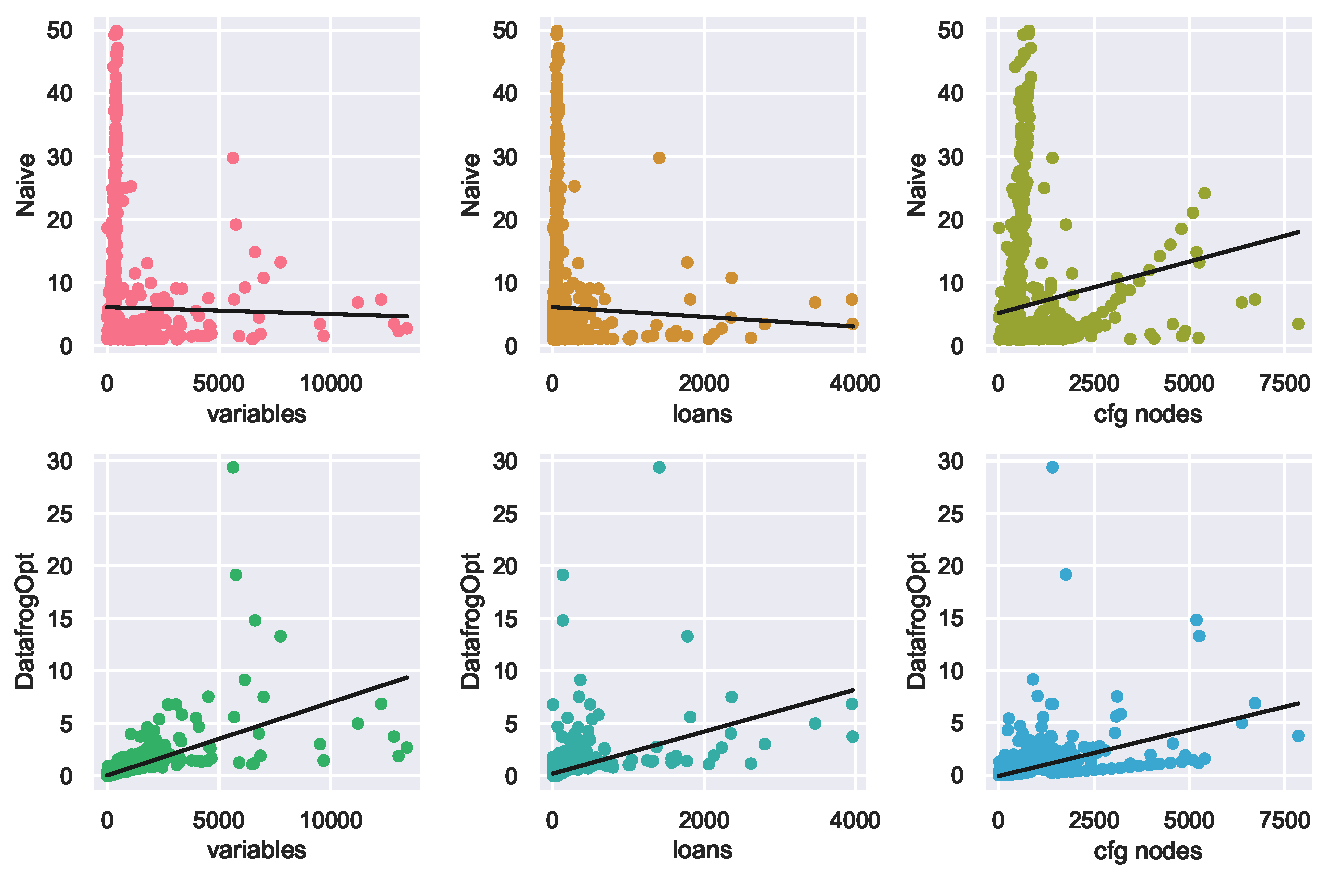
\includegraphics[width=0.9\linewidth]{Graphs/corr_scatter.pdf}
  \caption{Scatter plot of solvetimes under the naive and optimised algorithms
    compared to variables and CFG edge count after having pruned extreme values
    (runtimes below 1~s or above 13~minutes).}
  \label{fig:input-scatter}
\end{figure}

% discuss the results and what that means for Polonius

\section{Optimising the Borrow Checker}\label{sec:optim-borr-check}

% known problem with large static arrays

% implied constraints, symmetries, optimisations

\chapter{Conclusions and Future Work}\label{cha:conclusions}
%\epigraph{\fixme{short quote}}

%\begin{appendices}
%\end{appendices}

%\backmatter
\printbibliography[heading=bibintoc]
\end{document}